% Preamble
\documentclass{article}
\setlength\parindent{0pt}

% Packages
\usepackage{amsmath}
\usepackage{textcomp}
\usepackage{multirow}
\usepackage{algorithm}
\usepackage{algpseudocode}
\usepackage{tikz}
\usepackage[linktocpage]{hyperref}

\hypersetup{
    colorlinks   = true,
    urlcolor     = blue,
    linkcolor    = blue,
    citecolor   = red
}

\title{\textbf{ScreenView Protocol}}
\author{Josh Brown}

% Document
\begin{document}
    \maketitle

    \begin{abstract}
        ScreenView is suite of cryptographical and application level networking protocols culminating to create a
        zero configuration end to end encrypted remote screen viewing and controlling software. ScreenView aims to
        replace TeamViewer, RDP, and VNC for many use cases while being more performant and more secure. ScreenView
        requires little setup an is just as easy or easier than other solutions. ScreenView defines four different
        layers of protocols, each encapsulating all the layers below it. Cryptography for communication between peers
        and the server is based upon TLS 1.3 and Wireguard. End-to-end cryptography used for ALL communication between
        peers is based upon TLS-SRP. ScreenView end-to-end cryptography prevents man-in-the-middle attacks even if
        the intermediary server is compromised, unlike TeamViewer. Screen data is sent over UDP to achieve superior
        performance than TCP based solutions such as VNC. All UDP packets must be authenticated with keys established
        over TCP before a response is made by the server preventing amplification attacks. A congestion control
        mechanism is used to handle low bandwidth and poor networking conditions. Finally, ScreenView supports
        advanced use cases including file transfer, multiple displays, sharing specific windows, shared whiteboards,
        and clipboard transfer.
    \end{abstract}

    \newpage

    \tableofcontents
    \newpage


    \section{Definitions}

    The key words "MUST", "MUST NOT", "REQUIRED", "SHALL", "SHALL NOT",
    "SHOULD", "SHOULD NOT", "RECOMMENDED", "MAY", and "OPTIONAL" in this
    document are to be interpreted as described in \href{https://datatracker.ietf.org/doc/html/rfc2119}{RFC 2119}.

    \newpage


    \section{Introduction}

    This section describes the high level overview of ScreenView. Terms used in this section are defined in other
    sections.\\

    \subsection{Application Layers}

    The table belows is an abstract diagram of the different layers of ScreenView. Each layer encapsulates all the
    below layers.

    \begin{center}
        \begin{tabular}{|l|}
            \hline
            Transport Layer                                         \\
            | Server Encryption Layer                               \\
            || Server Communication Layer                           \\
            ||| E2EE (Peer $\leftrightarrow$ Peer) Encryption Layer \\
            |||| Host $\leftrightarrow$ Client Communication Layer  \\
            \hline
        \end{tabular}
    \end{center}

    The Transport Layer is the OSI Transport Layer level protocol for networking (TCP or UDP). The \hyperlink{section
    .3}{Server
    Encryption Layer} provides security between the Server and a Peer. \hyperlink{section.4}{The Server Communication
    Layer} facilities communication between Peers and the Client. The \hyperlink{section.5}{E2EE (Peer
        $\leftrightarrow$ Peer) Encryption Layer} provides end-to-end encryption between Peers and other Peers. The
    \hyperlink{section.6}{Host $\leftrightarrow$ Client Communication Layer} facilities communication between Peers.

    \subsection{Overview}

    To begin, a Peer connects to the server over TCP and commences the Server Encryption Layer protocol for TCP
    defined. Next the Server Communication Layer is used. All Server Communication Layer messages are encrypted,
    authenticated, and encapsulated in messages defined in
    the Server Encryption Layer. Once a session is established between two peers, the E2EE (Peer $\leftrightarrow$ Peer)
    Encryption Layer commences. All E2EE (Peer $\leftrightarrow$ Peer) Encryption messages are encapsulated in Server
    Communication Layer messages. Finally, the Host $\leftrightarrow$
    Client Communication Layer commences as defined in \hyperlink{section.6}{6}. All Host $\leftrightarrow$ Client
    Communication Layer messages are encrypted, authenticated, and encapsulated in E2EE (Peer $\leftrightarrow$ Peer)
    Encryption
    Layer messages.

    \subsection{Transport Messages Total Header Sizes}

    % TODO


    \section{Server Encryption Layer}

    The Server Encryption Layer provides security for communication between Peers and the Server. TCP and UDP have
    different security methods.

    \subsection{TCP}

    The TCP Server Encryption Layer is heavily based on a simplification of TLS 1.3 as defined in. % TODO defined in

    \subsubsection{PeerHello}

    \begin{center}
        Peer \textrightarrow\ Server\\
        \begin{tabular}{|c|c|c|}
            \hline
            \textbf{Bytes} & \textbf{Name} & \textbf{Value} \\
            \hline
            1              & type          & 1              \\
            \hline
            16             & public-key    &                \\
            \hline
        \end{tabular}
    \end{center}

    \begin{align*}
        &(E_{peer}^{pub},\,E_{peer}^{priv}) := \text{DH-Generate()}\\
        &\text{public-key} := E_{peer}^{pub}
    \end{align*}

    \subsubsection{ServerHello}

    \begin{center}
        Server \textrightarrow\ Peer\\
        \begin{tabular}{|c|c|c|}
            \hline
            \textbf{Bytes}             & \textbf{Name}       & \textbf{Value} \\
            \hline
            1                          & type                & 2              \\
            \hline
            3                          & certificates-length &                \\
            \hline
            \emph{certificates-length} & certificate\_list   &                \\
            \hline
            16                         & public-key          &                \\
            \hline
            variable                   & certificate-verify  &                \\
            \hline
        \end{tabular}
    \end{center}

    certificate\_list is defined in \href{https://datatracker.ietf.org/doc/html/rfc8446#section-4.4.2}{RFC8446
    Section-4.4.2}.

    \begin{align*}
        & (E_{serv}^{pub},\, E_{serv}^{priv}) := \text{DH-Generate()}\\
        & \text{public-key} := E_{serv}^{pub}
    \end{align*}

    certificate-verify is defined in \href{https://datatracker.ietf.org/doc/html/rfc8446#section-4.4
.3}{RFC8445 Section-4.4.3} with the following modification. The content that is signed is:\\

    \begin{align*}
        \text{content} := \text{``SreenViewServerVerify''}\ ||\ 0\ ||\ E_{serv}^{pub}
    \end{align*}

    The Client MUST validate all signatures in accordance with the TLS spec.

    \subsubsection{Transport Data Key Derivation}

    \begin{align*}
        & C_{peer} = \text{DH}(E_{serv}^{pub},\ E_{peer}^{priv})\\
        & C_{serv} = \text{DH}(E_{peer}^{pub},\ E_{serv}^{priv})\\
        & (T_{peer}^{send} = T_{serv}^{recv},\ T_{peer}^{recv} = T_{serv}^{send}) := \text{KDF}_2(C_{peer} = C_{serv},
        \ \epsilon) \\
        & N_{peer}^{send} = N_{serv}^{recv} = N_{peer}^{recv} = N_{serv}^{send} := 0
    \end{align*}

    \subsubsection{Subsequent Messages: Transport Data Messages}

    \begin{center}
        Peer $\leftrightarrow$ Server\\
        \begin{tabular}{|c|c|c|}
            \hline
            \textbf{Bytes}     & \textbf{Name} & \textbf{Value} \\
            \hline
            1                  & type          & 3              \\
            \hline
            2                  & data-length   &                \\
            \hline
            \emph{data-length} & data          &                \\
            \hline
        \end{tabular}
    \end{center}

    \begin{align*}
        & \text{data} := \text{AEAD}(T_{m}^{send}, N_{m}^{send}, P, \epsilon) \\
        & N_{m}^{send} := N_{m}^{send} + 1
    \end{align*}

    $N_{m}$ is an 64 bit counter that MUST NOT wrap. After a transport message is sent, if $N_{m}$ equals
    ($2^{64}-1$) the TCP connection MUST be dropped. Subsequent TCP messages MUST NOT be sent. \\

    Where $P$ is the payload to be transported

    \subsection{UDP}

    UDP encryption and authentication rely on the \emph{session-id}, \emph{peer-id} and \emph{peer-key} values
    established in a session
    (described in \hyperlink{subsection.5.4}{5.4}). The Server MUST NOT
    process or reply to any messages that don't pass authentication. This prevents an amplification attack.\\
    % TODO Consider IP address stuff

    \subsubsection{Transport Data Key Derivation}

    \begin{align*}
        &  G:= \text{session-id}                                                               \\
        &  H := \text{peer-id}                                                                \\
        &  J := \text{peer-key}                                                              \\
        &  (V_{peer}^{send} = V_{serv}^{recv}, V_{peer}^{recv} = V_{serv}^{send}) := \text{KDF}_2(\text{HASH}(G\,
        ||\, H\,||\, J), \epsilon)                                        \\
        &   M_{peer}^{send} = M_{serv}^{recv} = M_{peer}^{recv} = M_{serv}^{send} := 0
    \end{align*}

    \subsubsection{Transport Data Messages}

    \begin{center}
        Peer \textrightarrow Server\\
        \begin{tabular}{|c|c|c|}
            \hline
            \textbf{Bytes}                & \textbf{Name}  & \textbf{Value} \\
            \hline
            1                             & type           & 4              \\
            \hline
            16                            & \emph{peer-id} &                \\
            \hline
            8                             & counter        &                \\
            \hline
            $\text{UDP length} - 8$ bytes & data           &                \\
            \hline
        \end{tabular}
    \end{center}

    \begin{center}
        Server \textrightarrow Peer\\
        \begin{tabular}{|c|c|c|}
            \hline
            \textbf{Bytes}                & \textbf{Name} & \textbf{Value} \\
            \hline
            1                             & type          & 5              \\
            \hline
            8                             & counter       &                \\
            \hline
            $\text{UDP length} - 8$ bytes & data          &                \\
            \hline
        \end{tabular}
    \end{center}


    \begin{align*}
        & \text{data} := \text{AEAD}(V_{m}^{send}, M_{m}^{send}, P, \epsilon)\\
        & \text{counter} := M_{m}^{send}\\
        & M_{m}^{send} := M_{m}^{send} + 1
    \end{align*}


    $M_{m}$ is an 64 bit counter that MUST NOT wrap. After a transport message is sent, if $M_{m}$ equals
    ($2^{64}-1$) the TCP connection MUST be dropped. Subsequent UDP messages MUST NOT be sent. \\

    Where $P$ is the payload to be transported


    \section{ScreenView Server Communication (SVSC) Protocol }

    The SVSC protocol is the Server Communication Layer protocol used for Peers to interact with the relay server,
    Server. Peers can lease an ID as well as begin a session with another Peer. Once a session is established, Peers can
    forward messages to another Peer. Unless otherwise noted, all messages MUST occur over TCP.\\

    With the exception of the \emph{Handshake} messages. All SVSC messages' first byte contain a number to indicate
    the message type.

    \subsection{Definitions}
    The following definitions are used globally throughout the document:

    \begin{itemize}
        \item Peer - denotes a client in classical server/client environment
        \item Server - The intermediary server used for routing and proxying data between
    \end{itemize}

    \subsection{Handshake}

    \subsubsection{ProtocolVersion}

    Handshaking begins by the Server sending the Peer a \emph{ProtocolVersion} message. This lets the server know
    the version supported by the Host.\\

    The \emph{ProtocolVersion} message consists of 12 bytes interpreted as a string of ASCII characters in the format
    "SVSC xxx.yyy" where xxx and yyy are the major and minor version numbers, padded with zeros.

    \begin{center}
        Server \textrightarrow\ Peer\\
        \begin{tabular}{|c|c|c|}
            \hline
            \textbf{Bytes} & \textbf{Name} & \textbf{Value}            \\
            \hline
            11             & version       & ``\texttt{SVSC 001.000}'' \\
            \hline
        \end{tabular}
    \end{center}

    The Peer replies back either \texttt{0} to indicate the version is not acceptable and that the handshake has
    failed or \texttt{1} if the version is acceptable to the Peer and the handshake as succeeded. If 0 is sent, all
    communication MUST cease and the TCP connection MUST be terminated.

    \begin{center}
        Peer \textrightarrow\ Server\\
        \begin{tabular}{|c|c|c|}
            \hline
            \textbf{Bytes} & \textbf{Name} & \textbf{Value} \\
            \hline
            1              & ok            & 0 or 1         \\
            \hline
        \end{tabular}
    \end{center}

    \subsection{Leasing}

    A lease is a temporary assignment of an ID to a Peer. The ID format and generation is discussed in
    \hyperlink{subsubsection.4.2.5}{4.2.5}. A maximum of 1 ID can be leased per TCP connection. ID generation MUST be
    rate limited to prevent ID exhaustion. Rate limiting rules are out of scope for this protocol, however some
    suggestions are listed in \hyperlink{subsubsection.4.2.6}{4.2.6}.

    \subsubsection{LeaseRequest}

    A \emph{LeaseRequest} message requests a lease of an ID.

    \begin{center}
        Peer \textrightarrow\ Server\\
        \begin{tabular}{|c|c|c|}
            \hline
            \textbf{Bytes} & \textbf{Name} & \textbf{Value} \\
            \hline
            1              & type          & 1              \\
            \hline
            1              & has-cookie    & 0 or 1         \\
            \hline
            \multicolumn{3}{|c|}{\textbf{Below only if \emph{has-cookie} is 1} } \\
            \hline
            24             & cookie        &                \\
            \hline
        \end{tabular}
    \end{center}

    If a Peer would like to request an ID it had previously been issued after expiration, it may include the cookie
    value it received in the \emph{LeaseResponse}.

    \subsubsection{LeaseResponse}

    A \emph{LeaseResponse} message is a response to a \emph{LeaseRequest}.

    If \emph{has-cookie} is 1, a Server MAY consider the \emph{cookie} value in \emph{LeaseRequest} or completely
    ignore it.

    \begin{center}
        Server \textrightarrow\ Peer\\
        \begin{tabular}{|c|c|c|}
            \hline
            \textbf{Bytes} & \textbf{Name} & \textbf{Value} \\
            \hline
            1              & type          & 2              \\
            \hline
            1              & accepted      & 0 or 1         \\
            \hline
            \multicolumn{3}{|c|}{\textbf{Below only if \emph{accepted} is 1} } \\
            \hline
            4              & id            &                \\
            \hline
            24             & cookie        &                \\
            \hline
            8              & expiration    &                \\
            \hline
        \end{tabular}
    \end{center}

    \emph{expiration} is a 64 bit Unix timestamp representing the expiry of lease. Disconnection of a Peer (e.g,
    the TCP connection is dropped) does not end a lease.\\

    \emph{cookie} a 128 bit value. The generation of this value is discussed in \hyperlink{subsubsection.4.2.7}{4.2
    .7}.\\

    Consideration of the \emph{cookie} value MUST have no effect on the the value of \emph{accepted}. That is, if the
    request is for a specific ID (implied by the presence of a cookie value and a \emph{has-cookie} value equal to 1
    in the \emph{LeaseRequest}) and the ID requested is not available, the Server SHOULD respond with a different
    available ID and an \emph{accepted} value of 1 (assuming an ID is available).\\

    \emph{accepted} SHOULD only be 0 if no IDs are left or for rate limiting reasons.

    \subsubsection{LeaseExtensionRequest}

    A \emph{LeaseExtensionRequest} message is used to extend a lease. Before a lease has expired, the Peer can
    request a lease extension. The server can accept or deny this request.

    \begin{center}
        Peer \textrightarrow\ Server\\
        \begin{tabular}{|c|c|c|}
            \hline
            \textbf{Bytes} & \textbf{Name} & \textbf{Value} \\
            \hline
            1              & type          & 3              \\
            \hline
            24             & cookie        &                \\
            \hline
        \end{tabular}
    \end{center}

    \subsubsection{LeaseExtensionResponse}

    A \emph{LeaseExtensionResponse} message is a response to a \emph{LeaseExtensionRequest}.

    \begin{center}
        Server \textrightarrow\ Peer\\
        \begin{tabular}{|c|c|c|}
            \hline
            \textbf{Bytes} & \textbf{Name}  & \textbf{Value} \\
            \hline
            1              & type           & 4              \\
            \hline
            1              & extended       & 0 or 1         \\
            \hline
            \multicolumn{3}{|c|}{\textbf{Below only if \emph{extended} is 1} } \\
            \hline
            8              & new-expiration &                \\
            \hline
        \end{tabular}
    \end{center}

    \emph{new-expiration} is a 64 bit Unix timestamp representing the expiry of lease.

    \subsubsection{ID Generation}

    An ID is a 26 to 33 bit decimal number. This comes out to about up to 8 to 10 decimal digits, respectively. The
    Server may scale the keyspace depending on current usage. For optimal user experience while maintaining
    efficiency, the Server MUST only use keyspaces between 26 bits and 33 bits for ID generation. ID generation must
    also be uniformly random. All active IDs must be stored on the server. ID generation MAY occur using the below
    algorithm:\\

    Let $S$ represents a set of all active IDs, $B$ be a number of bits between 26 and 33, and $generate(x)$ be a
    functions that returns a $x$ uniformly random bits.

    \begin{algorithm}
        \caption{ID generation}
        \begin{algorithmic}
            \State $id$
            \Repeat
                \State $id\gets generate(B)$
            \Until{$id\notin S$}
            \State $S\gets S\cup \{id\}$
            \State \textbf{return} $id$
        \end{algorithmic}
    \end{algorithm}

    \subsubsection{Rate Limits}

    To prevent ID exhaustion, rate limits SHOULD be in place. TCP is used for \emph{LeaseRequests} so IP addresses
    can not be spoofed. However, using proxy services such as Tor, simple IP based rate limits are likely not
    entirely sufficient. Servers MAY want to block all known proxy IP addresses. Additionally, a Server MAY only want
    to allow one active ID per Peer.

    \subsubsection{Cookie Value}

    A \emph{cookie} value is a 128 bit value used for authentication in \emph{LeaseExtensionRequest} and
    \emph{LeaseRequest} messages. Specific generation of a \emph{cookie} is out of scope, however care must be taken
    to ensure it is not predictable or exploitable. This value MAY be simply a random 24 byte key, HMAC-SHA1($id$,
    $key$) $||$ $id$, or something else entirely.

    \subsection{Sessions}

    A session is a connection between two Peers. At least one Peer must have an ID. A Peer can have a maximum of one
    session at any time. Immediately after receiving a \emph{EstablishSessionResponse} message with a \emph{status}
    of 0 or a \emph{EstablishSessionNotification} message a Peer MUST establish UDP connection by sending a
    \emph{Keepalive} message as defined in \hyperlink{subsection.5.5}{5.5}. Failure to do so MAY result in dropped
    \emph{SessionData*} packets.

    \subsubsection{EstablishSessionRequest}

    An \emph{EstablishSessionRequest} message is a Peer request to establish a connection to a Peer.

    \begin{center}
        Peer \textrightarrow\ Server\\
        \begin{tabular}{|c|c|c|c|}
            \hline
            \textbf{Bytes} & \textbf{Name} & \textbf{Value} & \textbf{Description}                                 \\
            \hline
            1              & type          & 5              &                                                      \\
            \hline
            4              & lease-id      &                & The ID of the Peer to establish this connection with \\
            \hline
        \end{tabular}
    \end{center}

    \subsubsection{EstablishSessionResponse}

    An \emph{EstablishSessionResponse} message is a response to \emph{EstablishSessionRequest}.

    \begin{center}
        Server \textrightarrow\ Peer\\
        \begin{tabular}{|c|c|c|c|}
            \hline
            \textbf{Bytes} & \textbf{Name} & \textbf{Value} & \textbf{Description}                       \\
            \hline
            1              & type          & 6              &                                            \\
            \hline
            4              & lease-id      &                & the ID of the Peer attempted to connect to \\
            \hline
            1              & status        & 0-5            & described below                            \\
            \hline
            \multicolumn{4}{|c|}{\textbf{Below only if \emph{status} is 0} } \\
            \hline
            16             & session-id    &                & described below                            \\
            \hline
            16             & peer-id       &                & described below                            \\
            \hline
            16             & peer-key      &                & described below                            \\
            \hline
        \end{tabular}
    \end{center}

    \emph{status} can have the following values:

    \begin{center}
        \begin{tabular}{|c|c|}
            \hline
            \textbf{Value} & \textbf{Description}                 \\
            \hline
            0              & session establishment was successful \\
            \hline
            1              & ID not found                         \\
            \hline
            2              & Peer is offline                      \\
            \hline
            3              & Peer is busy                         \\
            \hline
            4              & You are busy                         \\
            \hline
            5              & Other error                          \\
            \hline
        \end{tabular}
    \end{center}

    A Peer may be considered offline if, for example, an unexpired ID has been assigned to them and then the TCP
    connection is dropped. Keepalive messages and timeouts are discussed in % TODO
    .\\

    \emph{session-id} is a 128 bit random value used for session identification\\

    \emph{peer-id} is a 128 bit random value used to authentication a peer for a given session.\\

    \subsubsection{EstablishSessionNotification}

    A \emph{EstablishSessionNotification} notifies a Peer that a session has been established with them.

    \begin{center}
        Server \textrightarrow\ Host\\
        \begin{tabular}{|c|c|c|c|}
            \hline
            \textbf{Bytes} & \textbf{Name} & \textbf{Value} & \textbf{Description}                                \\
            \hline
            1              & type          & 7              &                                                     \\
            \hline
            16             & session-id    &                & described in \hyperlink{subsubsection.4.3.2}{4.3.2} \\
            \hline
            16             & peer-id       &                & described in \hyperlink{subsubsection.4.3.2}{4.3.2} \\
            \hline
            16             & peer-key      &                & described in \hyperlink{subsubsection.4.3.2}{4.3.2} \\
            \hline
        \end{tabular}
    \end{center}

    \subsubsection{SessionEnd}

    A \emph{SessionEnd} message is used to terminate a session. Once a Server receives a \emph{SessionEnd} message,
    % // TODO

    \begin{center}
        Peer \textrightarrow\ Server\\
        \begin{tabular}{|c|c|c|c|}
            \hline
            \textbf{Bytes} & \textbf{Name} & \textbf{Value} & \textbf{Description} \\
            \hline
            1              & type          & 8              &                      \\
            \hline
        \end{tabular}
    \end{center}

    \subsubsection{SessionEndNotification}

    A \emph{SessionEndNotification} notifies a Peer that a session has ended. If a Client sends a \emph{SessionEnd}
    message, the Server MUST send a \emph{SessionEndNotification} message to a Host.

    \begin{center}
        Server \textrightarrow\ Peer\\
        \begin{tabular}{|c|c|c|c|}
            \hline
            \textbf{Bytes} & \textbf{Name} & \textbf{Value} & \textbf{Description} \\
            \hline
            1              & type          & 9              &                      \\
            \hline
        \end{tabular}
    \end{center}

    \subsubsection{SessionDataSend - TCP/UDP}

    A \emph{SessionDataSend} is a message from a Peer intended to be forwarded to the Peer on the other side of the
    session. If a connection is not available (e.g. UDP was dropped or never established) for
    \emph{SessionDataReceive} message to be sent to the other Peer, the
    \emph{SessionDataSend} message is silently dropped.

    \begin{center}
        Peer \textrightarrow\ Server\\
        \begin{tabular}{|c|c|c|c|}
            \hline
            \textbf{Bytes} & \textbf{Name} & \textbf{Value} & \textbf{Description}           \\
            \hline
            1              & type          & 10             &                                \\
            \hline
            3              & data-length   &                & length of the content in bytes \\
            \hline
            data-length    & data          &                & data to be forwarded           \\
            \hline
        \end{tabular}
    \end{center}

    \subsubsection{SessionDataReceive - TCP/UDP}

    A \emph{SessionDataReceive} is a message being forwarded to a Peer from the Peer on the other side of the
    session. The Server SHOULD forward the message along the same transport as it was received.

    \begin{center}
        Server \textrightarrow\ Peer\\
        \begin{tabular}{|c|c|c|c|}
            \hline
            \textbf{Bytes} & \textbf{Name} & \textbf{Value} & \textbf{Description}           \\
            \hline
            1              & type          & 11             &                                \\
            \hline
            3              & data-length   &                & length of the content in bytes \\
            \hline
            data-length    & data          &                & data to be forwarded           \\
            \hline
        \end{tabular}
    \end{center}

    \subsection{Keepalive - TCP/UDP}

    For each transport (TCP and UDP), if no message has been sent in \emph{KeepaliveTimeout} a Server sends a keepalive
    message over the respective transport. The Peer MUST respond with another Keepalive message.\\

    For TCP, if a \emph{KeepaliveTimeout} response is not received by the Server in
    double \emph{KeepaliveTimeout} seconds the TCP connection is considered dropped.\\

    For UDP, if a \emph{KeepaliveTimeout} response is not received by the Server in
    half  \emph{KeepaliveTimeout} seconds another \emph{Keepalive} message is sent. If a response is not received in
    an additional half \emph{KeepaliveTimeout} seconds, the UDP connection is considered dropped.

    \begin{center}
        Server $\leftrightarrow$ Peer\\
        \begin{tabular}{|c|c|c|c|}
            \hline
            \textbf{Bytes} & \textbf{Name} & \textbf{Value} \\
            \hline
            1              & type          & 0              \\
            \hline
        \end{tabular}
    \end{center}


    \section{Weak Pre Shared Key, Key Authentication (WPSKKA) Protocol}

    The WPSKKA protocol is the E2EE Encryption layer protocol used to communicate between peers. All WPSKKA messages'
    first byte contain a number to indicate
    the message type.\\

    WPSKKA relies on SRP as defined in \href{RFC5054}{https://datatracker.ietf.org/doc/html/rfc5054} to establish a
    shared key used to authenticate DH keys. The Host will serve as the SRP server, the client will serve as the SRP
    client.\\

    \begin{center}
        Host \textrightarrow\ Client\\
        \begin{tabular}{|c|c|c|}
            \hline
            \textbf{Bytes} & \textbf{Name} & \textbf{Value} \\
            \hline
            1              & type          & 1              \\
            \hline
            16             & username      &                \\
            \hline
            16             & salt          &                \\
            \hline
            256            & srp-B         &                \\
            \hline
            16             & public-key    &                \\
            \hline
        \end{tabular}
    \end{center}

    \begin{align*}
        & \text{SRP-HOST-INIT()}\\
        & (D_{host}^{pub},\, D_{host}^{priv}) := \text{DH-Generate()}\\
        & I := RAND(128)\\
        & s := RAND(128)\\
        & B := \text{SRP-B()}\\
        & username := I\\
        & salt := s\\
        & srp-B := B\\
        & \text{public-key} := C_{serv}^{pub}\\
    \end{align*}

    \begin{center}
        Client \textrightarrow\ Host\\
        \begin{tabular}{|c|c|c|}
            \hline
            \textbf{Bytes} & \textbf{Name} & \textbf{Value} \\
            \hline
            1              & type          & 2              \\
            \hline
            256            & srp-A         &                \\
            \hline
            16             & public-key    &                \\
            \hline
            32             & mac           &                \\
            \hline
        \end{tabular}
    \end{center}

    \begin{align*}
        & \text{SRP-CLIENT-INIT()}\\
        & (D_{client}^{pub},\, D_{client}^{priv}) := \text{DH-Generate()}\\
        & A := \text{SRP-A()}\\
        & L_{client} = L_{host} := \text{SRP-PREMASTER()}\\
        & \text{public-key} := \text{HMAC}(\text{KDF}_1(D_{client}^{pub}, L_{client}))\\
    \end{align*}

    \begin{center}
        Host \textrightarrow\ Client\\
        \begin{tabular}{|c|c|c|}
            \hline
            \textbf{Bytes} & \textbf{Name} & \textbf{Value} \\
            \hline
            1              & type          & 3              \\
            \hline
            32             & mac           &                \\
            \hline
        \end{tabular}
    \end{center}

    \begin{align*}
        & \text{mac} := \text{HMAC}(\text{KDF}_1(C_{host}^{pub}, L_{host}))\\
    \end{align*}

    \subsection{Transport Data Key Derivation}

    \begin{align*}
        & D_{host} = \text{DH}(D_{client}^{pub},\ D_{host}^{priv})\\
        & D_{client} = \text{DH}(D_{host}^{pub},\ D_{client}^{priv})\\
        & (U_{peer}^{send} = U_{serv}^{recv},\ U_{peer}^{recv} = U_{serv}^{send}) := \text{KDF}_2(D_{host} = D_{client},
        \ \epsilon) \\
        & O_{host}^{send} = O_{client}^{recv} = O_{host}^{recv} = O_{client}^{send} := 0
    \end{align*}

    \subsubsection{Subsequent Messages: Transport Data Messages}

    \begin{center}
        Host $\leftrightarrow$ Client\\
        \begin{tabular}{|c|c|c|}
            \hline
            \textbf{Bytes}     & \textbf{Name} & \textbf{Value} \\
            \hline
            1                  & type          & 4              \\
            \hline
            8                  & counter       &                \\
            \hline
            2                  & data-length   &                \\
            \hline
            \emph{data-length} & data          &                \\
            \hline
        \end{tabular}
    \end{center}

    \begin{align*}
        & \text{data} := \text{AEAD}(U_{m}^{send}, O_{m}^{send}, P, \epsilon)\\
        & \text{counter} := O_{m}^{send}\\
        & O_{m}^{send} := O_{m}^{send} + 1
    \end{align*}

    $O_{m}$ is an 64 bit counter that MUST NOT wrap. After a transport message is sent, if $O_{m}$ equals
    ($2^{64}-1$) the TCP connection MUST be dropped. Subsequent messages MUST NOT be sent. \\


    Where \emph{P} is the payload to be transported


    \section{Remote Visual Display (RVD) Protocol}

    The RVD protocol is used to communicate mouse input, keyboard input, frame data, and clipboard data between the
    Host and the Client.\\

    All messages MUST occur over the transport listed.\\

    With the exception of the \emph{Handshake} messages, all RVD messages' first byte contain a number to indicate
    the message type. \\

    A \emph{sequence-number} is an incrementing 32-bit counter each UDP message sent, separate for Host and Client. All
    messages sent over UDP MUST begin with a 4 bytes \emph{sequence-number}. \emph{sequence-number} is initialized
    to 0 and increments once for every UDP message sent by the respective Peer. Therefore each RVD UDP message looks
    like:

    \begin{center}
        \begin{tabular}{|c|c|}
            \hline
            \textbf{Bytes} & \textbf{Name}   \\
            \hline
            4              & sequence-number \\
            \hline
            variable       & RVD message     \\
            \hline
        \end{tabular}
    \end{center}

    \subsection{Combining Messages}

    In some situations, such as when a large screen change occurs or when the screen is first sent to the client,
    large amounts of \emph{FrameData}'s may need to be sent in quick succession. Often individual \emph{FrameData}'s
    will be much smaller than the MTU. Similar to TCP's Nagle algorithm, multiple UDP messages can be combined into a
    single UDP packet as long as the total size is remains less than the MTU. Each message directly follows the
    previous message with the first message directly following the sequence number. Only one \emph{sequence-number}
    is used:

    \begin{center}
        \begin{tabular}{|c|c|}
            \hline
            \textbf{Bytes} & \textbf{Name}   \\
            \hline
            4              & sequence-number \\
            \hline
            variable       & RVD message 1   \\
            \hline
            variable       & RVD message 2   \\
            \hline
            \hline
            variable       & etc.            \\
            \hline
        \end{tabular}
    \end{center}

    \subsection{Definitions}

    \begin{itemize}
        \item Host - A peer with an ID that wants to share their screen to the Client
        \item Client - A peer that wants to view and maybe control the Host's screen
        \item Display - A rectangular visual region that is shared by a Host to a Client. May or may not be
        \item \emph{Controllable}.
        \item Controllable - A \emph{Display} that accepts keyboard and mouse input.
    \end{itemize}

    \subsection{Handshake}

    \subsubsection{ProtocolVersion - TCP}
    Handshaking begins by the Host sending the client a \emph{ProtocolVersion} message. This lets the Client know the
    verison supported by the Host.\\

    The \emph{ProtocolVersion} message consists of 11 bytes interpreted as a string of ASCII characters in the format
    "RVD xxx.yyy" where xxx and yyy are the major and minor version numbers, padded with zeros.

    \begin{center}
        Host \textrightarrow\ Client\\
        \begin{tabular}{|c|c|c|}
            \hline
            \textbf{Bytes} & \textbf{Name} & \textbf{Value}           \\
            \hline
            11             & version       & ``\texttt{RVD 001.000}'' \\
            \hline
        \end{tabular}
    \end{center}

    The Client replies back either \texttt{0} to indicate the version is not acceptable and that the handshake has
    failed or \texttt{1} if the version is acceptable to the Client and the handshake as succeeded. If 0 is sent, all
    communication MUST cease and an error SHOULD be displayed to user. A \emph{SessionEnd} message should be sent by
    the Client. % TODO hyper

    \begin{center}
        Client \textrightarrow\ Host\\
        \begin{tabular}{|c|c|c|}
            \hline
            \textbf{Bytes} & \textbf{Name} & \textbf{Value} \\
            \hline
            1              & ok            & 0 or 1         \\
            \hline
        \end{tabular}
    \end{center}

    \subsubsection{Initialization}

    Once the handshake has succeeded the Host responds with a \emph{DisplayChange} message.

    \subsection{Control messages}
    Control messages are messages that instruct client about changes regarding the Host.

    \subsubsection{DisplayChange - TCP}
    A \emph{DisplayChange} message informs the client about the available \emph{Display}s. RVD supports up to 255
    displays.

    \begin{center}
        Host \textrightarrow\ Client\\
        \begin{tabular}{|c|c|c|}
            \hline
            \textbf{Bytes} & \textbf{Name}        & \textbf{Value}            \\
            \hline
            1              & type                 & 1                         \\
            \hline
            1              & clipboard-readable   & 0 or 1                    \\
            \hline
            1              & number-of-displays   & 1 - 255                   \\
            \hline
            variable       & displays-information & \emph{DisplayInformation} \\
            \hline
        \end{tabular}
    \end{center}

    Each \emph{Display} has an associated \emph{DisplayInformation}. \emph{displays-information} contains
    \emph{number-of-displays} \emph{DisplayInformation}'s. A \emph{DisplayInformation} is defined below:

    \begin{center}
        \begin{tabular}{|c|c|c|}
            \hline
            \textbf{Bytes}     & \textbf{Name} & \textbf{Description}                                 \\
            \hline
            1                  & display-id    &                                                      \\
            \hline
            2                  & width         & number of pixels of the width of this display        \\
            \hline
            2                  & height        & number of pixels of the width of this display        \\
            \hline
            2                  & cell-width    & number of pixels of the height of a cell in the grid \\
            \hline
            2                  & cell-height   & number of pixels of the height of a cell in the grid \\
            \hline
            1                  & access        & defined below                                        \\
            \hline
            1                  & name-length   & length of the \emph{display-name} in bytes           \\
            \hline
            \emph{name-length} & display-name  & the display name (UTF-8)                             \\
            \hline
        \end{tabular}
    \end{center}

    \textbf{Restrictions:}

    \begin{itemize}
        \item \emph{cell-width} MUST be less than \emph{width}. \emph{cell-height} must be less than \emph{height}.\\
        % // TODO define more restrictions %
        \item The \emph{access} byte defines what type of access is available for the display. The bits of the
        \emph{access} byte are described below in little endian.
    \end{itemize}


    \begin{center}
        \begin{tabular}{|c|c|}
            \hline
            \textbf{Bit} & \textbf{Name}                               \\
            \hline
            0            & Flush                                       \\
            \hline
            1            & \emph{Controllable}                         \\
            \hline
            2            & \multirow{6}{10em}{Reserved for future use} \\
            3            &                                             \\
            4            &                                             \\
            5            &                                             \\
            6            &                                             \\
            7            &                                             \\
            \hline
        \end{tabular}
    \end{center}

    If the \emph{Controllable} bit is 1 and the \emph{clipboard-readable} byte is set to 1, then the clipboard is
    writable. The \emph{Controllable} bit SHOULD be consistent throughout all displays.\\

    The \emph{Flush} bit indicates whether this display has changed, specifically if this \emph{display-id} refers to
    a different \emph{Display} than the same \emph{display-id} did in the previous \emph{DisplayChange} message. In
    initialization, this MUST always be 1 (as there is no previous \emph{DisplayChange}). If the display hasn't
    changed (0) then the frame data may be maintained. If \emph{Flush} is 0, \emph{width}, \emph{height} MUST remain
    the same as the previous \emph{DisplayChange} specified for the \emph{display-id}.\\


    Display cell numbering is right to left, up to down, 0 indexed as seen below. If $\text{cell-width}\ \%\
    \text{width} > 0$ the right column's width will be $\text{width}\ \%\ \text{cell-width}$. If $\text{height}\
    \%\ \text{cell-height} > 0$ the bottom row's height will be $\text{height}\ \%\ \text{cell-height}$.

    \begin{center}
        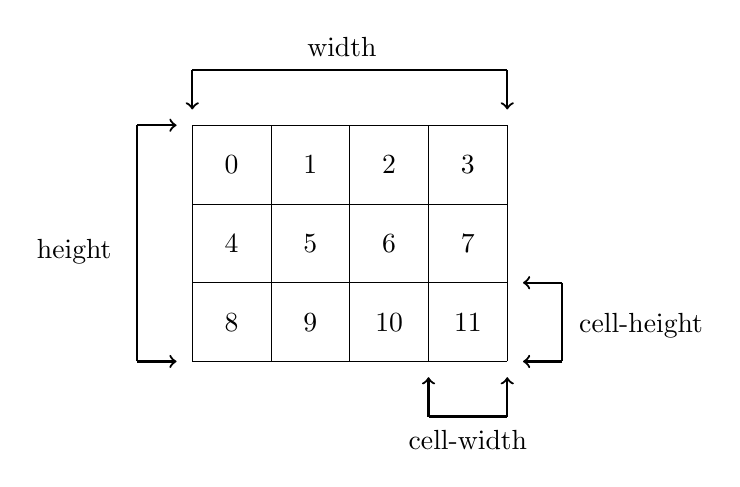
\begin{tikzpicture}
            \draw[step=1cm,black,very thin] (0,0) grid (4,3);
            \draw[thick,->] (-0.7,3) -- (-0.2,3);
            \draw[thick] (-0.7,3) -- (-0.7,0);
            \draw[thick,->] (-0.7,0) -- (-0.2,0);
            \draw (-1.5,1.4) node{height};

            \draw[thick,->] (0,3.7) -- (0,3.2);
            \draw[thick] (0,3.7) -- (4,3.7);
            \draw[thick,->] (4,3.7) -- (4,3.2);
            \draw (1.9,4) node{width};

            \draw[thick,->] (4.7,1) -- (4.2,1);
            \draw[thick] (4.7,1) -- (4.7,0);
            \draw[thick,->] (4.7,0) -- (4.2,0);
            \draw (5.7,0.45) node{cell-height};

            \draw[thick,->] (3,-0.7) -- (3,-0.2);
            \draw[thick] (3,-0.7) -- (4,-0.7);
            \draw[thick,->] (4,-0.7) -- (4,-0.2);
            \draw (3.5, -1) node{cell-width};

            \draw (0.5, 2.5) node{0};
            \draw (1.5, 2.5) node{1};
            \draw (2.5, 2.5) node{2};
            \draw (3.5, 2.5) node{3};

            \draw (0.5, 1.5) node{4};
            \draw (1.5, 1.5) node{5};
            \draw (2.5, 1.5) node{6};
            \draw (3.5, 1.5) node{7};

            \draw (0.5, 0.5) node{8};
            \draw (1.5, 0.5) node{9};
            \draw (2.5, 0.5) node{10};
            \draw (3.5, 0.5) node{11};
        \end{tikzpicture}
    \end{center}

    \subsubsection{DisplayChangeReceived - TCP}

    The \emph{DisplayChangeReceived} message is sent in reply after receiving a \emph{DisplayChange} message. It
    indicates to the Host they may start sending \emph{FrameData} referencing the new \emph{DisplayInformation} in
    the most recent \emph{DisplayChange}.

    \begin{center}
        Client \textrightarrow\ Host\\
        \begin{tabular}{|c|c|c|}
            \hline
            \textbf{Bytes} & \textbf{Name} & \textbf{Value} \\
            \hline
            1              & type          & 2              \\
            \hline
        \end{tabular}
    \end{center}

    \subsubsection{MouseLocation - TCP/UDP}

    The \emph{MouseLocation} message send information about where the mouse is currently on the screen.
    The Host sends this information periodically throughout the session.
    The Host SHOULD send a \emph{MouseLocation} update when mouse input is received from the Host's system or in
    reply when it receives a \emph{MouseInput}.

    \begin{center}
        Host \textrightarrow\ Client\\
        \begin{tabular}{|c|c|c|c|}
            \hline
            \textbf{Bytes} & \textbf{Name} & \textbf{Value} & \textbf{Description}      \\
            \hline
            3              & type          & 3              &                           \\
            \hline
            1              & display-id    & 0-255          &                           \\
            \hline
            2              & x-location    &                & x coordinate of the mouse \\
            \hline
            2              & y-location    &                & y coordinate of the mouse \\
            \hline
        \end{tabular}
    \end{center}

    \subsection{Input}

    Input messages (including \emph{MouseLocation}) may be sent over TCP or UDP. TCP is preferred in most situations.
    However, in situations where speed is prioritized over the guarantees TCP provides (such as gaming), UDP can be
    used.

    \subsubsection{MouseInput - TCP/UDP}

    \begin{center}
        Client \textrightarrow\ Host\\
        \begin{tabular}{|c|c|c|c|}
            \hline
            \textbf{Bytes} & \textbf{Name} & \textbf{Value} & \textbf{Description}      \\
            \hline
            1              & type          & 4              &                           \\
            \hline
            1              & display-id    & 0-255          &                           \\
            \hline
            2              & x-position    &                & x coordinate of the mouse \\
            \hline
            2              & y-position    &                & y coordinate of the mouse \\
            \hline
            1              & button-mask   &                & described below           \\
            \hline
        \end{tabular}
    \end{center}

    %  https://github.com/rfbproto/rfbproto/blob/master/rfbproto.rst#pointerevent %
    Indicates either pointer movement or a pointer button press or release. The pointer is now at (x-position,
    y-position), and the current state of buttons 1 to 8 are represented by bits 0 to 7 of button-mask respectively,
    0 meaning up, 1 meaning down (pressed).\\

    On a conventional mouse, buttons 1, 2 and 3 correspond to the left, middle and right buttons on the mouse. On a
    wheel mouse, each step of the wheel is represented by a press and release of a certain button. Button 4 means up,
    button 5 means down, button 6 means left and button 7 means right.

    \subsubsection{KeyInput - TCP/UDP}

    The \emph{KeyInput} event sends key presses or releases.

    \begin{center}
        Client \textrightarrow\ Host\\
        \begin{tabular}{|c|c|c|c|}
            \hline
            \textbf{Bytes} & \textbf{Name} & \textbf{Value} & \textbf{Description}                                 \\
            \hline
            1              & type          & 5              &                                                      \\
            \hline
            1              & down-flag     & 0 or 1         & indicates whether the key is now pressed or released \\
            \hline
            4              & key           &                & "keysym"                                             \\
            \hline
        \end{tabular}
    \end{center}

    Details can be found at the \href{https://github.com/rfbproto/rfbproto/blob/master/rfbproto.rst#keyevent}{RFB Spec}

    \subsection{Clipboard} % // TODO this needs to be worked on

    \subsubsection{ClipboardTypeRequest - TCP}

    Used to request clipboard types the Host supports.

    \begin{center}
        Client \textrightarrow\ Host\\
        \begin{tabular}{|c|c|c|}
            \hline
            \textbf{Bytes} & \textbf{Name} & \textbf{Value} \\
            \hline
            1              & type          & 6              \\
            \hline
        \end{tabular}
    \end{center}

    \subsubsection{ClipboardTypeResponse - TCP}

    Response to the \emph{ClipboardTypeRequest}

    \begin{center}
        Host \textrightarrow\ Client\\
        \begin{tabular}{|c|c|c|c|}
            \hline
            \textbf{Bytes} & \textbf{Name}             & \textbf{Value} & \textbf{Description} \\
            \hline
            1              & type                      & 7              &                      \\
            \hline
            1              & number-of-clipboard-types & 0-255          &                      \\
            \hline
            variable       & data (variable bytes)     &                & described below      \\
            \hline
        \end{tabular}
    \end{center}

    \emph{number-of-clipboard-types} is always 0 if \emph{clipboard-readable} is 0.\\

    \emph{data} contains \emph{number-of-clipboard-types} \emph{ClipboardType}s. \emph{ClipboardType} is defined below.

    \begin{center}
        \begin{tabular}{|c|c|c|c|}
            \hline
            \textbf{Bytes}     & \textbf{Name} & \textbf{Value} & \textbf{Description} \\
            \hline
            1                  & type-length   & 1-255          &                      \\
            \hline
            \emph{type-length} & type-name     &                & type name in ASCII   \\
            \hline
        \end{tabular}
    \end{center}

    \subsubsection{CopyRequest - TCP}

    This is a request for a keyboard contents. It can be made by either the Client or the Host.

    \begin{center}
        Client $\leftrightarrow$ Host\\
        \begin{tabular}{|c|c|c|c|}
            \hline
            \textbf{Bytes}     & \textbf{Name} & \textbf{Value} & \textbf{Description} \\
            \hline
            1                  & type          & 8              &                      \\
            \hline
            1                  & type-length   & 1-255          &                      \\
            \hline
            \emph{type-length} & type-name     &                & type name in ASCII   \\
            \hline
        \end{tabular}
    \end{center}

    \subsubsection{CopyResponse - TCP}

    \emph{CopyResponse} message is a response to a \emph{CopyRequest}.

    \begin{center}
        Client $\leftrightarrow$ Host\\
        \begin{tabular}{|c|c|c|c|}
            \hline
            \textbf{Bytes}        & \textbf{Name} & \textbf{Value} & \textbf{Description} \\
            \hline
            1                     & type          & 9              &                      \\
            \hline
            1                     & accepted      & 0 or 1         &                      \\
            \hline
            \multicolumn{4}{|c|}{\textbf{Below only if \emph{accepted} is 1} } \\
            \hline
            1                     & type-length   & 1-255          &                      \\
            \hline
            \emph{type-length}    & type-name     &                & type name in ASCII   \\
            \hline
            3 & content-length & & the length of the content  (maximum $2^{24}$
            bytes or ~16MB ) \\
            \hline
            \emph{content-length} & data          &                & zlib'ed raw data     \\
            \hline
        \end{tabular}
    \end{center}



    \emph{accepted} indicates whether the \emph{CopyRequest} was accepted. If 0, the rest of the message MUST not exist.
    If \emph{clipboard-readable} is 0, \emph{accepted} is always 0. A Client or Host may send this message without a
    request.
    If a \emph{CopyResponse} is unsolicited, then \emph{accepted} MUST be 1.\\

    \emph{data} is zlib compressed.

    \subsubsection{A note on Pasting}

    There is a no paste message. To paste data an unsolicited \emph{CopyResponse} may be sent and then the keyboard
    shortcut (ctrl+v or cmd+v) should be sent via the \emph{KeyboardMessage}

    \subsection{FrameData - UDP}
    The \emph{FrameData} message contains an update of a particular cell on a particular \emph{Display}.

    \begin{center}
        Host \textrightarrow Client\\
        \begin{tabular}{|c|c|c|}
            \hline
            \textbf{Bytes} & \textbf{Name} & \textbf{Value} \\
            \hline
            1              & type          & 10             \\
            \hline
            4              & frame-number  &                \\
            \hline
            1              & display-id    & 0-255          \\
            \hline
            2              & cell-number   &                \\
            \hline
            2              & size          &                \\
            \hline
            \emph{size}    & data          &                \\
            \hline
        \end{tabular}
    \end{center}

    \emph{frame-number} is a 32 bit counter, initialized with 0 at the begining of the protocol, and incremented once
    from \emph{FrameData} message sent.

    \emph{data} contains jpeg pixel data of the updated cell.

    \subsection{Congestion}

    When sending messages over a network the network may become congested to avoid congesting the network further RVD
    implements a congestion detection and congestion control mechanism. RVD uses Additive increase/multiplicative
    decrease or AIMD to control the \emph{OutputMaximum} which is the maximum messages allowed per
    \emph{CongestionWindow}.

%    \subsubsection{QoSMessage - TCP}
%
%    \begin{center}
%        Client $\leftrightarrow$ Host\\
%        \begin{tabular}{|c|c|c|}
%            \hline
%            \textbf{Bytes} & \textbf{Name}   & \textbf{Value} \\
%            \hline
%            1              & type            & 11             \\
%            \hline
%            4              & sequence-number &                \\
%            \hline
%        \end{tabular}
%    \end{center}

\end{document}
